\newpage
\section{Frameworks}
\label{frameworks}
\subsection{Introduction}
A framework is \textit{\say{a supporting structure around which something can be built}} \cite{FrameworkDefinition}, and can be used in connection with securing the \acrshort{sdlc}. Frameworks outlined in this chapter are not intended to be rigid regulations but rather valuable recommendations for software developers to enhance security measures. By implementing these suggestions, developers can confidently improve the security of their software.

\subsection{Supply-chain Levels for Software Artifacts}
\label{Supply-chainLevelsforSoftwareArtifacts}
\acrlong{slsa} (\acrshort{slsa})\footnote{Available at: \url{https://slsa.dev/}} is a framework for securing the software supply chain created by Google in collaboration with OpenSSF\footnote{Available at: \url{https://openssf.org/}} \cite{SLSAgeneral}. The framework is made into a common vocabulary checklist for developers to evaluate the security of the software they are creating. \acrshort{slsa} is organized into tracks and levels. The levels refer to the increasing security guarantee of the supply chain, the highest level being level 3. The levels are split further into tracks. Tracks are certain aspects of the supply chain, for example, the Build track, which currently is \acrshort{slsa}s only track. 

\vspace{2mm}
\begin{figure}[H]
    \centering
    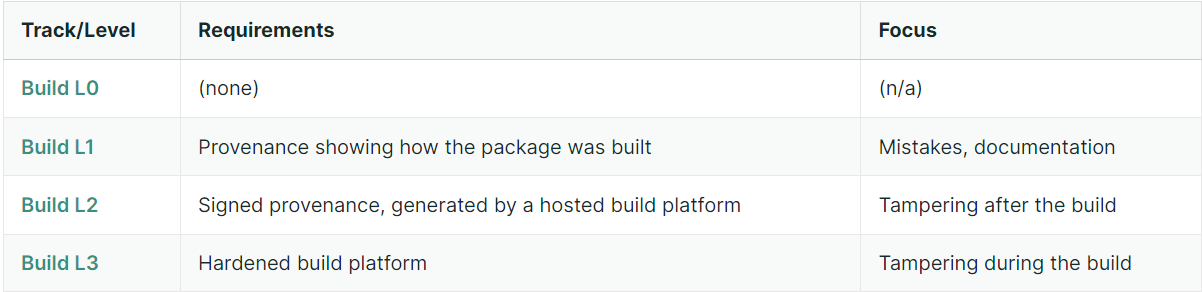
\includegraphics[width=0.8\columnwidth]{Images/slsalevels.png}
    \caption{\acrshort{slsa} levels for the Build track}\cite{SLSAlevels}
    \label{fig: SLSA levels for the Build track}
\end{figure}
Currently, there are three levels split into one track. To achieve the different build levels, the developers have to do the following:
\\~\\
To achieve \acrshort{slsa} Build Level 1, the developers must use a consistent build process, which can quickly be adopted. Additionally, it is essential to generate \gls{provenance} automatically on the build platform, which describes how the artifact was built. This includes information on the entity responsible for building the package, the specific build process used, and the top-level inputs utilized during the build process.
\\~\\
In order to reach \acrshort{slsa} Level 2, all Level 1 requirements must be in place. Further, the build has to be run on a platform that signs the \gls{provenance}. Finally, this \gls{provenance}'s authenticity must also be verified.
\\~\\
Similarly to Level 2, all previous level requirements must be achieved to get to \acrshort{slsa} Level 3. In addition, the build platform needs to be able to secure the secrets used for signing \gls{provenance} and prevent any interference between runs from the same project.  


\subsection{Secure Software Development Framework}
\label{ssdf}
\acrlong{ssdf} (\acrshort{ssdf})\footnote{Available at: \url{https://csrc.nist.gov/Projects/ssdf}} is a framework consisting of practices for a secure software development, created by \acrlong{nist} (\acrshort{nist}). The organization should integrate the \acrshort{ssdf} into their already existing software development practices. \acrshort{ssdf} does not specify how each practice should be implemented. It emphasizes the outcome of the practices rather than how to perform them. Organizations in any sector or community can use the \acrshort{ssdf}, regardless of their size or level of cyber security competence. This framework is intended to be user-friendly and adaptable, making it appropriate for a wide range of businesses with varied levels of cyber security knowledge. Organizations can use the \acrshort{ssdf} to adopt secure software development practices and reduce the risk of potential security vulnerabilities. The framework does not introduce new practices or define new terminology. However, it presents a set of high-level practices based on known standards, guidelines, and documents relevant to secure software development practices. 
\\~\\
The benefits of describing the practices at a high level include that they can be used by organizations in every industry and community, despite their size or level of cyber security knowledge. It can also help companies that buy and use software understand the secure software development methods used by their suppliers. All the practices are described in the framework\footnote{Latest version: \url{https://nvlpubs.nist.gov/nistpubs/SpecialPublications/NIST.SP.800-218.pdf}}.
\\~\\
There are four groups into which the practices are divided \cite{ssdf}:
\begin{itemize}
  \item \textbf{Prepare the Organization (PO)}: \textit{\say{Organizations should ensure that their people, processes, and technology are prepared to perform secure software development at the organization level. Many organizations will find some PO practices to also apply to subsets of their software development, like individual development groups or projects.}}
  \item \textbf{Protect the Software (PS)}: \textit{\say{Organizations should protect all components of their software from tampering and unauthorized access.}}
  \item \textbf{Produce Well-Secured Software (PW)}: \textit{\say{Organizations should produce well-secured software with minimal security vulnerabilities in its releases.}}
  \item \textbf{Respond to Vulnerabilities (RV)}: \textit{\say{Organizations should identify residual vulnerabilities in their software releases and respond appropriately to address those vulnerabilities and prevent similar ones from occurring in the future.}}
\end{itemize}

Each practice definition has the following components \cite{ssdf}:
\begin{itemize}
  \item \textbf{Practice}: Name of the practice with a unique identifier, with a description. 
  \item \textbf{Task}: One or more steps may be required to carry out a procedure.
  \item \textbf{Notional Implementation Examples}: A selection of tools, procedures, or approaches is presented that may aid in the execution of tasks. It should be noted that these examples are not exhaustive, and their use is not obligatory. In addition, some examples may not be relevant to specific companies or circumstances.
  \item \textbf{References}: References towards established secure development practice documentation and their mappings to specific tasks. Not all references will be relevant in all cases of software development. 
\end{itemize}